% Final wrapper for Chapter 4. The v7 text remains the method source of truth; this layer adds final figure placement and implementation-level clarifications verified against the frozen v07 training script.
\begingroup
\newcount\ThesisChFourSubsec
\ThesisChFourSubsec=0
\let\ThesisChFourOriginalSubsection\subsection
\renewcommand{\subsection}[1]{%
  \advance\ThesisChFourSubsec by 1%
  \ifnum\ThesisChFourSubsec=3
    \ThesisChFourOriginalSubsection{#1}%
    为统一全文术语，后文将实测状态与健康参考之间的差异统称为状态残差，其中$e_i(t)$表示原量纲状态残差，$r_i(t)$表示经训练集统计量标准化后的状态残差，$R_t$表示连续时间位置组成的多参数状态残差窗口。%
  \else
    \ifnum\ThesisChFourSubsec=4
      为与实际训练实现保持一致，两层GCN编码后并非直接对全部节点做全局平均。本文将节点初始表示$H^{(0)}$与第二层图卷积表示$H^{(2)}$在特征维拼接，并进行LayerNorm：
      \begin{equation}
      H_{cat}=\mathrm{LN}\left(H^{(0)}\Vert H^{(2)}\right)\in\mathbb R^{N\times 2d},
      \end{equation}
      式中，$\Vert$表示特征维拼接。分类阶段按照固定DCS节点顺序将$H_{cat}$展平为$2Nd$维向量，再依次通过96维全连接层、ReLU、Dropout(0.05)和故障类别输出层。该节点保持式读出既保留原始局部状态，又保留两层知识拓扑传播后的结构信息，避免全局平均池化消除固定测点的物理身份。预训练阶段则由线性解码器将每个节点的$2d$维表示恢复至长度为$L_r$的残差窗口，仅在被遮蔽位置计算重构误差。
      \begin{figure}[htbp]
        \centering
        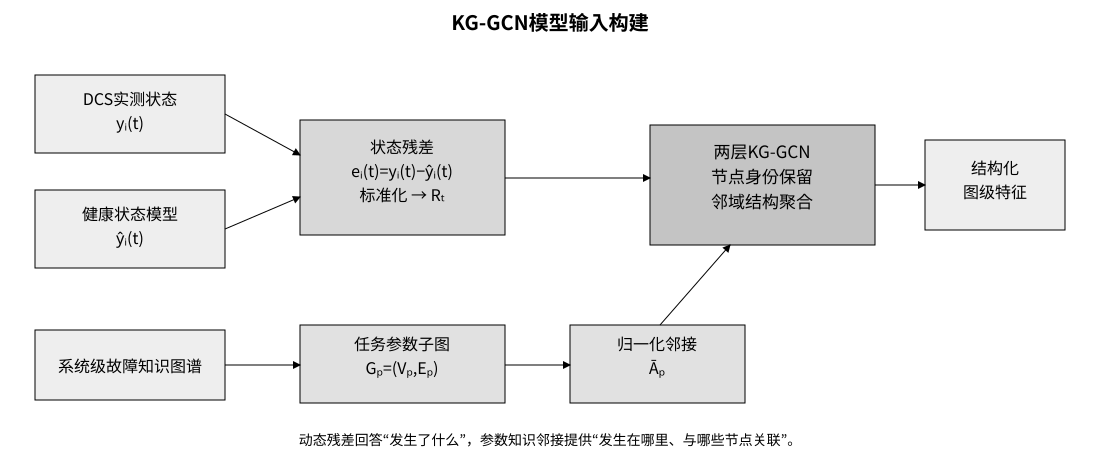
\includegraphics[width=0.98\textwidth]{figures/ch4/fig4_1_kg_gcn_input.pdf}
        \caption{KG-GCN模型输入构建过程}
        \label{fig:kg_gcn_input_final}
      \end{figure}
    \fi
    \ifnum\ThesisChFourSubsec=5
      \begin{figure}[htbp]
        \centering
        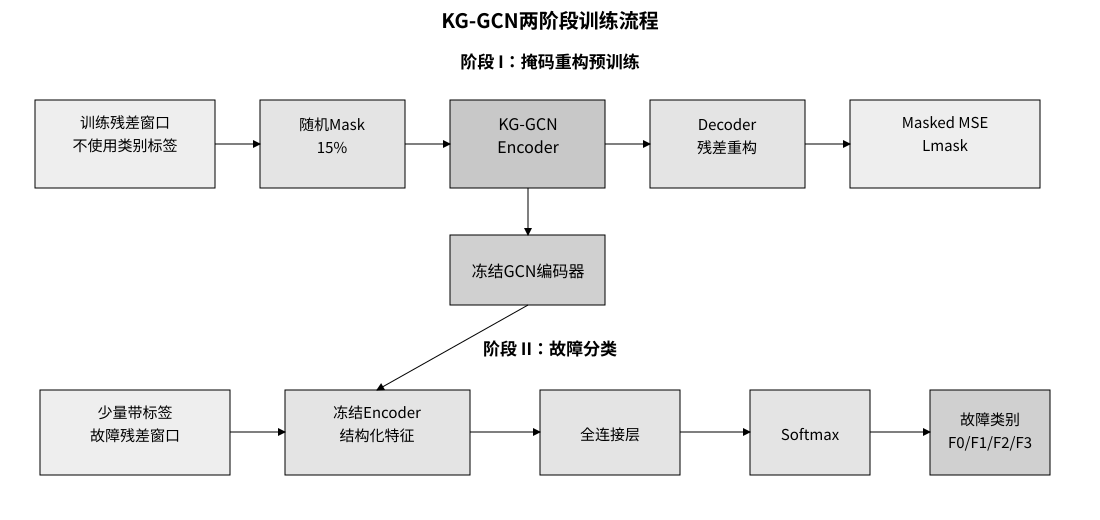
\includegraphics[width=0.98\textwidth]{figures/ch4/fig4_2_mask_training.pdf}
        \caption{KG-GCN掩码预训练与故障分类流程}
        \label{fig:mask_training_final}
      \end{figure}
    \fi
    \ThesisChFourOriginalSubsection{#1}%
  \fi
}
\section{基于KG-GCN的燃煤机组汽轮机系统故障诊断方法}
\label{sec:kg_gcn_v7}

\subsection{引言}

燃煤机组汽轮机系统故障具有多参数耦合和跨设备传播特征。传统阈值或经验规则方法依赖预先设定的异常判据，当运行边界变化或故障表现发生偏移时，其适应能力受到限制。纯数据驱动分类模型虽然能够学习复杂非线性特征，但通常将监测参数组织为规则向量或矩阵，参数之间的实际热力连接并未显式参与特征传播。当不同故障共享部分监测参数时，仅依赖局部数据特征容易出现类别混淆。

第三章构建的汽轮机系统故障知识图谱将设备、参数、异常和故障之间的关联组织为图结构，可为多参数诊断提供静态领域知识。第二章建立的健康状态模型则能够根据当前运行边界给出设备正常状态参考，并由实测状态与模型输出之间的偏差信息形成动态状态表征。本文将两类信息进行融合：以知识图谱投影得到的参数关系作为图结构，以状态监测偏差作为节点动态特征，通过GCN完成关联参数之间的信息聚合，并采用残差窗口遮蔽预训练提高少故障标签条件下的特征学习能力。

\subsection{图卷积网络}
\label{subsec:gcn_theory_v7}

汽轮机设备和参数之间构成由实际热力连接决定的非欧几里得拓扑。传统卷积运算依赖规则网格上的固定邻域，难以直接描述任意参数节点之间的连接关系。图卷积网络（Graph Convolutional Network，GCN）依据图邻接关系聚合节点自身及相邻节点特征，适合处理具有明确结构关系的工业过程数据\cite{Kipf2017GCN}。

设参数图为$G=(V,E)$，其中$V=\{v_1,v_2,\ldots,v_N\}$为参数节点集合，$E$为节点之间的关联边。图的拓扑由邻接矩阵$A\in\mathbb R^{N\times N}$表示。为使每次图卷积同时保留节点自身信息，在邻接矩阵中加入单位矩阵$I_N$：
\begin{equation}
\tilde A=A+I_N.
\end{equation}
式中，$\tilde A$为加入自连接后的邻接矩阵。相应度矩阵定义为
\begin{equation}
\tilde D_{ii}=\sum_j\tilde A_{ij}.
\end{equation}
在此基础上进行对称归一化，得到
\begin{equation}
\bar A=\tilde D^{-\frac{1}{2}}\tilde A\tilde D^{-\frac{1}{2}}.
\end{equation}
归一化处理可以减小不同节点度数差异对特征聚合幅值的影响。

设第$l$层节点特征矩阵为$H^{(l)}$，标准图卷积层的传播形式为
\begin{equation}
H^{(l+1)}=\sigma\left(\bar A H^{(l)}W^{(l)}\right),
\end{equation}
式中：$W^{(l)}$为第$l$层可学习权重矩阵；$\sigma(\cdot)$为非线性激活函数。每一层图卷积均按照邻接矩阵规定的连接路径，将目标节点及其邻域信息映射至新的特征空间。随着图卷积层数增加，节点能够逐步获得更远邻域内的关联信息。

本文采用两层GCN完成汽轮机参数关联信息聚合。考虑固定DCS参数自身状态同样具有诊断意义，在标准GCN基础上保留节点自身表示，并采用残差连接和LayerNorm抑制多层传播造成的局部信息衰减：
\begin{equation}
H^{(1)}=\mathrm{ReLU}\left[\mathrm{LN}\left(H^{(0)}+\bar A H^{(0)}W^{(1)}\right)\right],
\end{equation}
\begin{equation}
H^{(2)}=\mathrm{ReLU}\left[\mathrm{LN}\left(H^{(1)}+\bar A H^{(1)}W^{(2)}\right)\right].
\end{equation}
第一层聚合直接相邻参数信息，第二层进一步传递两跳邻域特征。由此，每个参数节点的表示同时包含自身动态变化和局部热力拓扑信息。

\subsection{KG-GCN模型输入构建}
\label{subsec:kg_input_v7}

第三章知识图谱包含设备、参数、异常、故障和处置等多种实体，而实时图卷积计算需要在参数节点上加载数值状态。因此，首先从系统级知识图谱中提取能够与实际DCS状态量建立映射的参数实体，并依据设备归属、介质流向和直接热力接口关系形成任务参数图。设任务参数图为
\begin{equation}
G_p=(V_p,E_p),
\end{equation}
式中：$V_p$为可加载实时状态的参数节点集合；$E_p$为由系统知识图谱投影得到的参数关联边。由$E_p$构建邻接矩阵$A_p$，并按前述方法得到归一化邻接矩阵$\bar A_p$。该矩阵在诊断过程中保持不变，用于规定不同参数之间的信息传播路径。

完成参数图构建后，将状态监测模型输出转化为动态节点特征。对于第$i$个状态参数，在时刻$t$的DCS实测值和健康状态模型输出分别记为$y_i(t)$和$\hat y_i(t)$，二者之间的状态偏差定义为
\begin{equation}
e_i(t)=y_i(t)-\hat y_i(t).
\end{equation}
在健康运行条件下，健康状态模型能够解释由负荷、入口边界和操作调节引起的大部分正常变化，$e_i(t)$主要反映预测误差和测量扰动；当设备状态发生异常时，实测状态相对于健康参考产生系统性偏离，相关参数的状态偏差随之发生变化。

由于不同参数的量纲和数值范围存在差异，对各参数状态偏差进行标准化：
\begin{equation}
r_i(t)=\frac{e_i(t)-\mu_i}{\sigma_i+\varepsilon},
\end{equation}
式中：$\mu_i$和$\sigma_i$分别为训练集第$i$个参数健康状态偏差的均值和标准差；$\varepsilon$为防止分母为零的微小常数。标准化统计量仅由训练数据计算，验证集和测试集不参与参数估计。

单一时刻全部参数的标准化状态偏差可写为
\begin{equation}
\mathbf r_t=[r_1(t),r_2(t),\ldots,r_N(t)]^{\mathrm T}.
\end{equation}
单时刻向量能够表示参数在当前时刻相对于健康参考的偏离，但无法描述故障随时间演化的连续特征。为此，对连续$L_r$个采样时刻进行滑动组织，构造参数--时间残差矩阵
\begin{equation}
R_t=
\begin{bmatrix}
r_1(t-L_r+1)&\cdots&r_1(t)\\
r_2(t-L_r+1)&\cdots&r_2(t)\\
\vdots&\ddots&\vdots\\
r_N(t-L_r+1)&\cdots&r_N(t)
\end{bmatrix}
\in\mathbb R^{N\times L_r}.
\end{equation}
式中，矩阵每一行固定对应一个参数节点，每一列对应一个连续时间位置。通过这种组织方式，多参数动态偏差被转化为能够与知识图谱节点一一对应的时序特征矩阵。

在GCN输入层中，首先将每个参数节点的时间窗口映射至$d$维初始特征空间：
\begin{equation}
H^{(0)}=\mathrm{ReLU}(R_tW_e+b_e),
\end{equation}
式中：$W_e\in\mathbb R^{L_r\times d}$和$b_e$分别为节点特征映射权重和偏置。随后，将节点初始特征$H^{(0)}$与知识图谱得到的归一化邻接矩阵$\bar A_p$共同输入GCN，实现动态运行信息在参数知识拓扑上的逐层传播。

固定DCS参数所在的物理位置本身具有诊断意义，因此本文在图级特征形成过程中保留节点顺序，不采用会完全消除节点身份的全局平均方式。最终图级特征同时包含节点局部状态和图卷积传播后的结构信息，并作为分类层输入。至此，知识图谱中的静态参数关系与状态监测模型产生的动态偏差信息被统一组织为KG-GCN的模型输入。

\subsection{KG-GCN模型训练}
\label{subsec:kg_training_v7}

故障类别标签通常需要依据运行记录、检修结论或人工确认获得，其获取成本明显高于一般运行状态数据。若直接使用有限的带标签故障样本训练全部图卷积参数，模型容易过度拟合已有故障模式。为减少对故障标签数量的依赖，本文采用两阶段训练方式：首先在不使用类别标签的残差窗口上进行掩码重构预训练，使GCN学习知识图谱约束下的参数关联；随后固定预训练后的图卷积编码器，仅利用带标签故障窗口训练分类层。

设预训练阶段使用的残差窗口集合为
\begin{equation}
\mathcal D_u=\{R^{(1)},R^{(2)},\ldots,R^{(M_u)}\},
\end{equation}
式中：$R^{(n)}$为第$n$个残差窗口；$M_u$为预训练窗口数量。预训练过程中随机遮蔽部分输入位置。设掩码矩阵为$M\in\{0,1\}^{N\times L_r}$，其中$M_{ij}=0$表示第$i$个参数在第$j$个时间位置被遮蔽，$M_{ij}=1$表示该位置保持可见，则遮蔽后的输入为
\begin{equation}
\tilde R=M\odot R+(1-M)\odot R_{mask}.
\end{equation}
式中：$\odot$表示逐元素乘法；$R_{mask}$表示遮蔽位置的替代值，本文取0。

将遮蔽后的残差窗口与参数邻接矩阵输入图卷积编码器：
\begin{equation}
Z=E_{\theta}(\bar A_p,\tilde R),
\end{equation}
式中：$E_{\theta}$为待预训练的GCN编码器；$\theta$为其中的可学习参数。编码器输出$Z$包含可见残差及其图邻域关联信息。随后通过解码器将结构化表示恢复至原始残差空间：
\begin{equation}
\hat R=D_{\phi}(Z),
\end{equation}
式中：$D_{\phi}$为解码器；$\phi$为解码器参数。

预训练阶段仅在被遮蔽位置计算重构误差：
\begin{equation}
\mathcal L_{mask}=\frac{\sum_{ij}(1-M_{ij})(R_{ij}-\hat R_{ij})^2}{\sum_{ij}(1-M_{ij})+\varepsilon}.
\end{equation}
通过最小化$\mathcal L_{mask}$，GCN编码器需要依据可见参数状态及其知识图谱邻域关系恢复缺失信息，从而在不使用故障类别标签的条件下学习多参数之间的结构化残差特征。

完成掩码预训练后，固定图卷积编码器参数，进入故障分类阶段。设带标签故障窗口样本集合为
\begin{equation}
\mathcal D_l=\{(R^{(n)},y^{(n)})\}_{n=1}^{M_l},
\end{equation}
式中：$R^{(n)}$为第$n$个故障残差窗口；$y^{(n)}$为对应故障类别标签；$M_l$为带标签故障样本数量。故障窗口经过预训练编码器后得到图级特征
\begin{equation}
\mathbf g^{(n)}=E_{\theta^*}(\bar A_p,R^{(n)}),
\end{equation}
式中：$\theta^*$表示预训练完成后固定的编码器参数。

分类层通过全连接映射和Softmax函数输出不同故障类别的预测概率：
\begin{equation}
\hat{\mathbf p}^{(n)}=\mathrm{Softmax}\left(W_c\mathbf g^{(n)}+b_c\right).
\end{equation}
式中：$W_c$和$b_c$分别为分类层权重和偏置。对于$C$类故障，分类阶段采用交叉熵损失函数
\begin{equation}
\mathcal L_{cls}=-\frac{1}{M_l}\sum_{n=1}^{M_l}\sum_{k=1}^{C}y_{nk}\log \hat p_{nk}.
\end{equation}
通过最小化$\mathcal L_{cls}$，分类层学习不同故障在图级残差特征空间中的判别边界。完成分类层训练后，新的残差窗口与参数邻接矩阵共同输入KG-GCN，即可获得相应故障类别概率。

\subsection{本章小结}

本章构建了基于知识图谱和图卷积网络的燃煤机组汽轮机系统故障诊断方法。首先介绍GCN在参数图上的特征传播过程，并采用两层图卷积聚合参数邻域信息；随后从第三章系统级知识图谱中抽取可与DCS状态量建立映射的参数关系，将第二章健康状态模型产生的多参数状态偏差组织为滑动时间窗口，与参数邻接矩阵共同形成KG-GCN输入；在模型训练阶段，首先在不使用类别标签的残差窗口上实施随机遮蔽重构预训练，随后固定图卷积编码器并利用带标签故障样本训练分类层。由此形成“知识图谱参数关系--状态监测偏差--图卷积特征传播--掩码预训练--故障分类”的诊断流程。下一章选取VHP作为代表性设备，对所提方法进行算例验证。
\endgroup
